
如果应用程序运行缓慢,那么很可能想知道代码中的时间都花费在什么地方了。在这种情况下,使用XRay检测代码会有所帮助。基本上,在每个函数的入口和出口,都会插入一个对运行时库的特殊调用。这允许计算函数被调用的频率,以及在函数中花费的时间。可以在llvm/lib/XRay/目录中找到Pass的实现,运行时是compiler-rt的一部分。\par

下面的示例源代码中,通过调用usleep()函数来模拟实际工作。函数的作用是:休眠10μs。func2()函数要么调用func1(),要么休眠100μs,这取决于n参数是奇数还是偶数。在main()函数中,两个函数都是在循环中调用的。在xraydemo.c文件中保存以下代码:\par

\begin{lstlisting}[caption={}]
#include <unistd.h>

void func1() { usleep(10); }

void func2(int n) {
	if (n % 2) func1();
	else usleep(100);
}

int main(int argc, char *argv[]) {
	for (int i = 0; i < 100; i++) { func1(); func2(i); }
	return 0;
}
\end{lstlisting}

要在编译期间启用XRay检测,需要指定-fxray-instrument选项,不测试小于200条指令的函数。这是一个由开发人员定义的任意阈值,在例子中,函数不会被检测。该阈值可以通过-fxrayin\allowbreak struction-threshold= 指定,或者可以添加一个function属性来控制函数是否应该检测,例如:添加以下修饰会让函数始终执行检测:\par

\begin{lstlisting}[caption={}]
void func1() __attribute__((xray_always_instrument));
\end{lstlisting}

同样,通过使用xray\underline{~}never\underline{~}instrument属性,可以关闭函数的检测功能。\par

现在,将使用命令行选项编译xraydemo.c文件:

\begin{tcolorbox}[colback=white,colframe=black]
\$ clang -fxray-instrument -fxray-instruction-threshold=1 -g $\setminus$ \\
\hspace*{1cm}xraydemo.c -o xraydemo
\end{tcolorbox}

现在,将使用命令行选项编译xraydemo.c文件在生成的二进制文件中,检测功能默认关闭。如果运行该二进制文件,您将不会注意到与未插装的二进制文件的区别。XRA\underline{~}OPTIONS环境变量用于控制运行时数据的记录。要启用数据收集,运行应用程序如下所示:\par

\begin{tcolorbox}[colback=white,colframe=black]
\$ XRAY\underline{~}OPTIONS= "patch\underline{~}premain=true xray\underline{~}mode=xray-basic "$\setminus$ \\
./xraydemo
\end{tcolorbox}

xray\underline{~}mode=xray-basic选项告诉运行时我们想要使用基本模式。在这种模式下,将收集所有的运行时数据,这可能生成巨大的日志文件。当给出patch\underline{~}premain=true选项时,那么在main()函数之前运行的函数也会被检测。\par

执行该命令后,将在收集的数据所在的目录中看到一个新文件,需要使用llvm-xray工具从这个文件中提取可读的信息。\par

llvm-xray工具支持各种子命令。可以使用account子命令提取一些基本统计信息,例如:要获得被调用最多的前10个函数,可以添加-top=10选项来限制输出,并添加-sort=count选项来指定函数调用计数作为排序标准。可以使用-sortorder=选项影响排序顺序。执行如下命令获取统计信息:\par

\begin{tcolorbox}[colback=white,colframe=black]
\$ llvm-xray account xray-log.xraydemo.xVsWiE -sort=count$\setminus$ \\
\hspace*{0.5cm}-sortorder=dsc -instr\underline{~}map ./xraydemo \\
Functions with latencies: 3 \\
\hspace*{0.5cm}funcid \hspace{1cm}count \hspace{2cm}sum \hspace{1cm}function \\
\hspace*{1.4cm}1\hspace{1.4cm}150\hspace{1.4cm}0.166002 \hspace{1cm}demo.c:4:0: func1 \\
\hspace*{1.4cm}2\hspace{1.4cm}100\hspace{1.4cm}0.543103 \hspace{1cm}demo.c:9:0: func2 \\
\hspace*{1.4cm}3\hspace{1.8cm}1 \hspace{1.3cm}0.655643 \hspace{1cm}demo.c:17:0: main
\end{tcolorbox}

可以看到,func1()函数调用得最频繁,以及在这个函数中花费的累计时间。这个示例只有三个函数,所以-top=在这里没有明显的效果,但对于实际应用程序来说,它非常有用。\par

从收集的数据中,可以重构运行时发生的所有堆栈帧。可以使用stack子命令查看排名前10的堆叠。为了简洁起见,此处显示的输出简化了:\par

\begin{tcolorbox}[colback=white,colframe=black]
\$ llvm-xray stack xray-log.xraydemo.xVsWiE -instr\underline{~}map$\setminus$ \\
\hspace*{0.5cm}./xraydemo \\
Unique Stacks: 3 \\
Top 10 Stacks by leaf sum:\\
\\
Sum: 1325516912\\
lvl \hspace{1cm}function \hspace{2.5cm}count \hspace{2.5cm}sum\\
\#0\hspace{1.5cm}main \hspace{3.3cm}1 \hspace{1.3cm}1777862705 \\
\#1\hspace{1.5cm}func2 \hspace{3.0cm}50 \hspace{1.35cm}1325516912 \\
\\
Top 10 Stacks by leaf count:\\
\\
Count: 100 \\
lvl \hspace{1cm}function \hspace{2.5cm}count \hspace{2.5cm}sum \\
\#0\hspace{1.5cm}main \hspace{3.3cm}1 \hspace{1.3cm}1777862705 \\
\#1\hspace{1.5cm}func1 \hspace{2.9cm}100 \hspace{1.45cm}303596276
\end{tcolorbox}

堆栈帧是一个函数调用的序列。func2()函数由main()函数调用,这是累积耗时最长的堆栈帧。深度取决于调用多少函数,堆栈帧通常很大。\par

这个子命令还可以用于从堆栈帧创建火焰图,可以很容易地识别哪些函数具有较大的累积运行时。输出是包含计数和运行时信息的堆栈帧。使用flamegraph.pl脚本,可以将数据转换为可缩放矢量图形(Scalable Vector Graphics, SVG)文件,并且可以在浏览器中查看该文件。\par

使用下面的命令,可以指示llvm-xray使用-all-stacks选项输出所有堆栈帧。使用-stack-format=\allowbreak flame选项,输出将以flamegraph.pl脚本所期望的格式显示。使用-aggregationtype选项,可以选择是按总时间还是按调用次数聚合堆栈帧。llvm-xray的输出通过管道传输到flamegraph.pl脚本中,结果输出保存在flame.svg文件中:\par

\begin{tcolorbox}[colback=white,colframe=black]
\$ llvm-xray stack xray-log.xraydemo.xVsWiE -all-stacks$\setminus$ \\
\hspace*{0.5cm}-stack-format=flame \verb|--|aggregation-type=time$\setminus$ \\
\hspace*{0.5cm}-instr\underline{~}map ./xraydemo | flamegraph.pl >flame.svg
\end{tcolorbox}

在浏览器中打开生成的flame.svg文件。图表如下所示:\par

\hspace*{\fill} \par %插入空行
\begin{center}
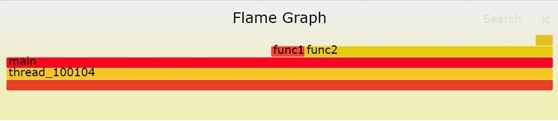
\includegraphics[width=1\textwidth]{content/3/chapter11/images/1.jpg}\\
图11.1 – 由llvm-x射线生成的火焰图
\end{center}

火焰图第一眼看起来可能会令人困惑,因为x轴没有通常的流逝时间的含义。相反,函数只是简单地按名称排序。颜色的选择要有良好的对比,没有其他意义。从上面的图中,可以很容易地确定调用层次结构和在函数中花费的时间。\par

只有将鼠标移到表示堆栈帧的矩形上,才会显示堆栈帧的相关信息。用鼠标单击框架,可以放大此堆栈框架。如果想要确定值得优化的函数,火焰图是很有帮助的。想了解更多关于火焰图的信息,请访问火焰图的作者Brendan Gregg的网站,\url{http://www.brendangregg.com/flamegraphs.html}。\par

您可以使用convert子命令将数据转换为.yaml格式或Chrome跟踪查看器可视化使用的格式。后者是另一种从数据创建图形的好方法。将数据保存在xray.evt文件中:\par

\begin{tcolorbox}[colback=white,colframe=black]
\$ llvm-xray convert -output-format=trace\underline{~}event$\setminus$ \\
\hspace*{0.5cm}-output=xray.evt -symbolize –sort$\setminus$ \\
\hspace*{0.5cm}-instr\underline{~}map=./xraydemo xray-log.xraydemo.xVsWiE
\end{tcolorbox}

如果不指定-symbolic选项,则结果图中不会显示函数名。\par

一旦完成,打开Chrome浏览器,输入Chrome:///跟踪。然后,点击加载按钮来加载xray.evt文件。您将看到以下可视化数据:\par

\hspace*{\fill} \par %插入空行
\begin{center}
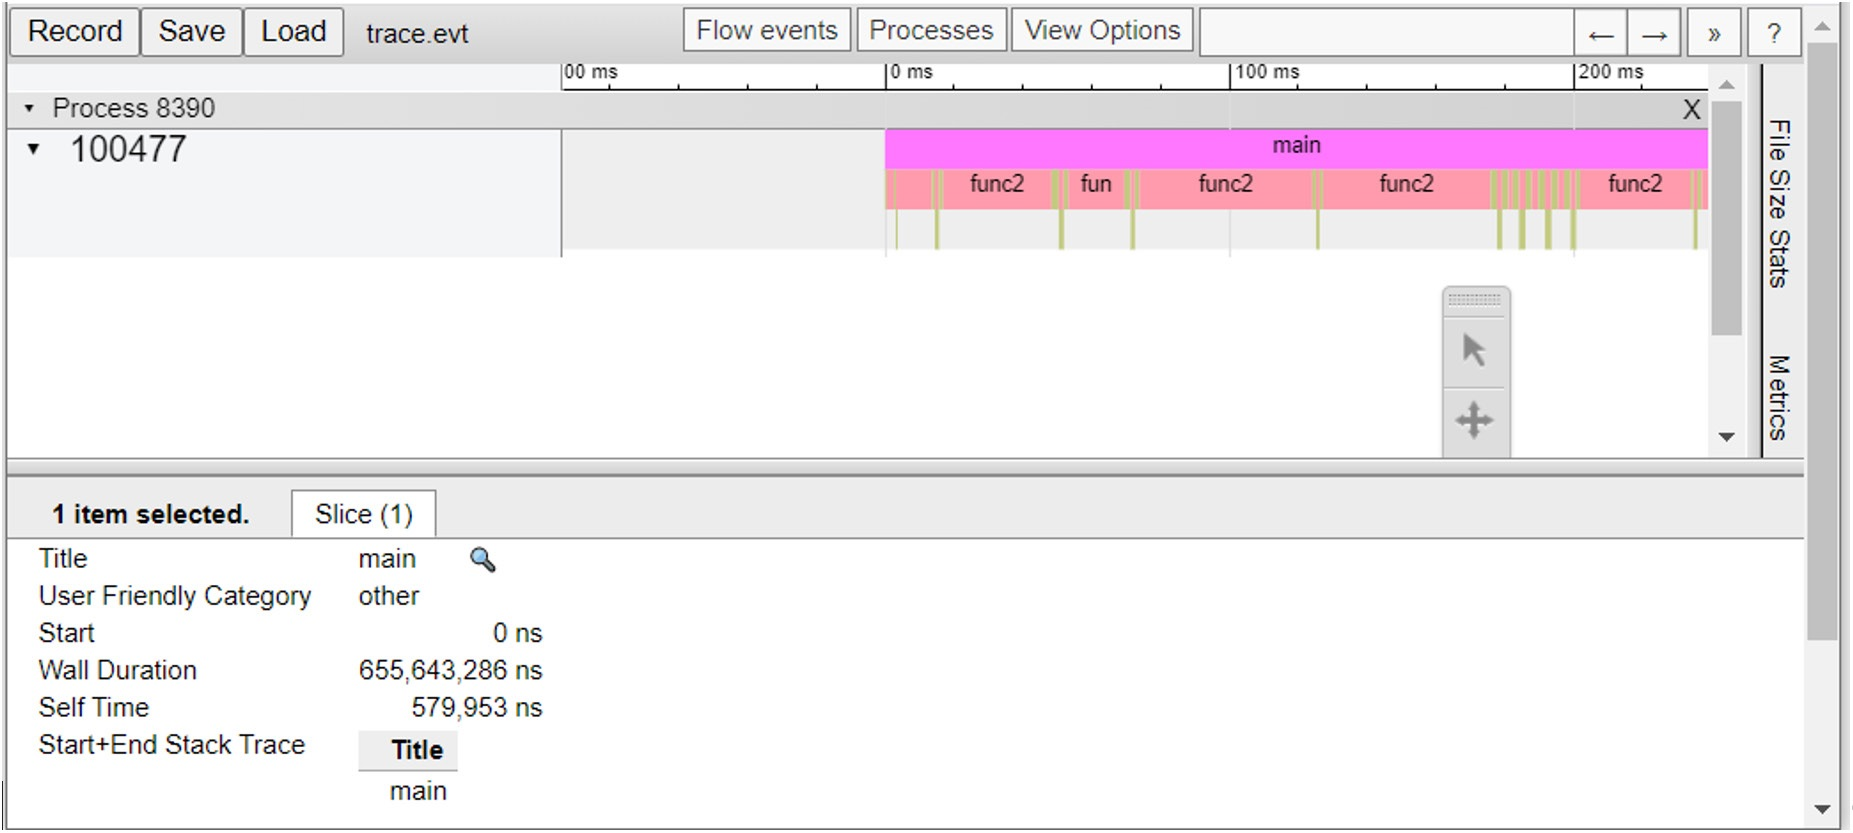
\includegraphics[width=1\textwidth]{content/3/chapter11/images/2.jpg}\\
图11.2 – Chrome跟踪查看器可视化生成的llvm-xray
\end{center}

在这个视图中,堆栈帧按函数调用发生的时间排序。关于可视化的进一步解释,请阅读教程 \url{https://www.chromium.org/developers/how-tos/trace-event-profiling-tool}。

\begin{tcolorbox}[colback=blue!5!white,colframe=blue!75!black, title=Tip]
llvm-xray工具有更多的功能。可以在LLVM网站上找到它,网址是\url{https://llvm.org/docs/XRay.html}和\url{https://llvm.org/docs/XRayExample.html}。
\end{tcolorbox}

本节中,我们学习了如何使用XRay检测应用程序,如何收集运行时信息,以及如何可视化数据。我们可以利用这些知识来发现应用程序中的性能瓶颈。\par

识别应用程序中的错误的另一种方法是通过静态分析器分析源代码。\par
















